% !TeX program = pdflatex
% Build (recommended):
%   pdflatex main.tex
%   biber main
%   pdflatex main.tex
%   pdflatex main.tex

\begin{filecontents*}{\jobname.bib}

% --- Author reference (blog article)
@online{delre_medallion_pdnd_2026,
  author  = {Del Re, Francesco},
  title   = {Medallion Architecture for PDND Interoperability Data in Public Administration},
  year    = {2026},
  month   = jan,
  url     = {https://engineering87.github.io/2026/01/18/medallion-architecture.html},
  note    = {Accessed: 2026-01-27}
}

% --- PDND primary references
@online{agid_pdnd_guidelines_2025,
  author  = {{Agenzia per l'Italia Digitale (AgID)}},
  title   = {Linee Guida sull'infrastruttura tecnologica della Piattaforma Digitale Nazionale Dati per l'interoperabilit\`a dei sistemi informativi e delle basi di dati (v2, maggio 2025)},
  year    = {2025},
  month   = jun,
  url     = {https://www.agid.gov.it/sites/agid/files/2025-06/Linee_guida_Infrastruttura_Interoperabilit\%C3\%A0_PDND_v2_maggio_2025.pdf},
  note    = {Accessed: 2026-01-27}
}

@online{pagopa_pdnd_guides,
  author  = {{PagoPA S.p.A.}},
  title   = {PDND Interoperability -- Guides (Developer Portal)},
  year    = {2025},
  url     = {https://developer.pagopa.it/pdnd-interoperabilita/guides},
  note    = {Accessed: 2026-01-27}
}

@online{developers_italia_pdnd,
  author  = {{Developers Italia}},
  title   = {PDND (Piattaforma Digitale Nazionale Dati) -- Overview},
  year    = {2026},
  url     = {https://developers.italia.it/it/pdnd/},
  note    = {Accessed: 2026-01-27}
}

% --- Legal / regulatory references (Once-Only, SDG)
@online{eu_reg_2018_1724,
  author  = {{European Union}},
  title   = {Regulation (EU) 2018/1724 establishing a Single Digital Gateway (Official Journal)},
  year    = {2018},
  month   = oct,
  url     = {https://eur-lex.europa.eu/eli/reg/2018/1724/oj/eng},
  note    = {Accessed: 2026-01-27}
}

@online{eu_impl_reg_2022_1463,
  author  = {{European Union}},
  title   = {Commission Implementing Regulation (EU) 2022/1463 on the Once-Only Technical System (OOTS) specifications (Official Journal)},
  year    = {2022},
  month   = aug,
  url     = {https://eur-lex.europa.eu/eli/reg_impl/2022/1463/oj/eng},
  note    = {Accessed: 2026-01-27}
}

@online{cad_normattiva,
  author  = {{Repubblica Italiana}},
  title   = {Decreto Legislativo 7 marzo 2005, n. 82 -- Codice dell'Amministrazione Digitale (CAD) -- Normattiva (testo vigente)},
  year    = {2005},
  url     = {https://www.normattiva.it/uri-res/N2Ls?urn:nir:stato:decreto.legislativo:2005-03-07;82=},
  note    = {Accessed: 2026-01-27}
}

@online{eidas_regulation_910_2014_pdf,
  author  = {{European Union}},
  title   = {Regulation (EU) No 910/2014 (eIDAS) on electronic identification and trust services -- Official Journal (PDF)},
  year    = {2014},
  url     = {https://eur-lex.europa.eu/legal-content/EN/TXT/PDF/?uri=CELEX\%3A32014R0910},
  note    = {Accessed: 2026-01-27}
}

% --- Medallion architecture (industry origin / popularization)
@online{databricks_medallion_docs,
  author  = {{Databricks}},
  title   = {What is the medallion lakehouse architecture?},
  year    = {2025},
  month   = sep,
  url     = {https://docs.databricks.com/aws/en/lakehouse/medallion},
  note    = {Accessed: 2026-01-27}
}

@online{databricks_medallion_glossary,
  author  = {{Databricks}},
  title   = {What is a Medallion Architecture?},
  year    = {2022},
  url     = {https://www.databricks.com/glossary/medallion-architecture},
  note    = {Accessed: 2026-01-27}
}

% --- Data quality foundations
@article{wang_strong_1996,
  author  = {Wang, Richard Y. and Strong, Diane M.},
  title   = {Beyond Accuracy: What Data Quality Means to Data Consumers},
  journal = {Journal of Management Information Systems},
  year    = {1996},
  volume  = {12},
  number  = {4},
  pages   = {5--33},
  doi     = {10.1080/07421222.1996.11518099}
}

@article{wand_wang_1996,
  author  = {Wand, Yair and Wang, Richard Y.},
  title   = {Anchoring Data Quality Dimensions in Ontological Foundations},
  journal = {Communications of the ACM},
  year    = {1996},
  volume  = {39},
  number  = {11},
  pages   = {86--95},
  url     = {https://web.mit.edu/tdqm/www/tdqmpub/WandWangCACMNov96.pdf},
  note    = {Accessed: 2026-01-27}
}

% --- Record linkage / entity resolution foundations
@article{fellegi_sunter_1969,
  author  = {Fellegi, Ivan P. and Sunter, Alan B.},
  title   = {A Theory for Record Linkage},
  journal = {Journal of the American Statistical Association},
  year    = {1969},
  volume  = {64},
  number  = {328},
  pages   = {1183--1210},
  doi     = {10.1080/01621459.1969.10501049}
}

% --- Semantic interoperability: Core Vocabularies / controlled vocabularies
@online{isa2_core_vocabularies,
  author  = {{European Commission (ISA$^2$)}},
  title   = {Core Vocabularies (solution overview)},
  year    = {2016},
  url     = {https://ec.europa.eu/isa2/solutions/core-vocabularies_en},
  note    = {Accessed: 2026-01-27}
}

@online{core_vocabularies_handbook_pdf,
  author  = {{European Commission (ISA$^2$)}},
  title   = {e-Government Core Vocabularies Handbook (PDF)},
  year    = {2016},
  url     = {https://ec.europa.eu/isa2/sites/default/files/e-government_core_vocabularies_handbook.pdf},
  note    = {Accessed: 2026-01-27}
}

@online{eu_vocabularies_controlled,
  author  = {{Publications Office of the European Union}},
  title   = {EU Vocabularies: Controlled vocabularies},
  year    = {2026},
  url     = {https://op.europa.eu/en/web/eu-vocabularies/controlled-vocabularies},
  note    = {Accessed: 2026-01-27}
}

% --- Ontology alignment (survey reference)
@article{granitzer_2010_ontology_alignment,
  author  = {Granitzer, Michael and Sabol, Vedran and Onn, Kok Wai and Lukose, Dickson and Tochtermann, Klaus},
  title   = {Ontology Alignment---A Survey with Focus on Visually Supported Semi-Automatic Techniques},
  journal = {Future Internet},
  year    = {2010},
  volume  = {2},
  number  = {3},
  pages   = {238--258},
  doi     = {10.3390/fi2030238},
  url     = {https://www.mdpi.com/1999-5903/2/3/238},
  note    = {Accessed: 2026-01-27}
}

\end{filecontents*}

\documentclass[11pt,a4paper]{article}

% --- Layout & typography
\usepackage[a4paper,margin=2.35cm]{geometry}
\usepackage[T1]{fontenc}
\usepackage[utf8]{inputenc}
\usepackage{lmodern}
\usepackage{microtype}
\usepackage{setspace}
\setstretch{1.07}

% --- Links & refs
\usepackage{hyperref}
\usepackage[nameinlink,noabbrev]{cleveref}
\hypersetup{
  colorlinks=true,
  linkcolor=blue,
  citecolor=blue,
  urlcolor=blue,
  pdftitle={Medallion Architecture for PDND: Data Quality, Integration, and Semantic Alignment},
  pdfauthor={Francesco Del Re}
}

% --- Lists
\usepackage{enumitem}
\setlist[itemize]{topsep=4pt,itemsep=2pt,parsep=0pt,leftmargin=1.2em}
\setlist[enumerate]{topsep=4pt,itemsep=2pt,parsep=0pt,leftmargin=1.4em}

% --- Figures & tables
\usepackage{graphicx}
\usepackage{booktabs}
\usepackage{caption}
\usepackage{adjustbox}
\usepackage{tabularx}

% --- TikZ (for a compact dataflow diagram)
\usepackage{tikz}
\usetikzlibrary{arrows.meta,positioning}

% --- Bibliography
\usepackage[
  backend=biber,
  style=ieee,
  sorting=none
]{biblatex}
\addbibresource{\jobname.bib}

% --- Code
\usepackage{listings}
\usepackage{xcolor}
\definecolor{codebg}{RGB}{248,248,248}
\definecolor{codeframe}{RGB}{220,220,220}

\lstdefinestyle{csharp}{
  backgroundcolor=\color{codebg},
  frame=single,
  rulecolor=\color{codeframe},
  basicstyle=\ttfamily\small,
  numbers=left,
  numberstyle=\scriptsize,
  numbersep=8pt,
  tabsize=2,
  breaklines=true,
  showstringspaces=false,
  upquote=true,
  captionpos=b,
  keywordstyle=\bfseries,
  commentstyle=\itshape,
  stringstyle=\ttfamily,
  morekeywords={record,init,required,async,await,ValueTask,DateOnly,DateTimeOffset},
}

% --- Sequence diagram
\usepackage{pgf-umlsd}

% In pgf-umlsd, \unitfactor is a NUMBER (TikZ assumes cm).
\makeatletter
\def\unitfactor{0.42}
\makeatother

% Patch pgf-umlsd \mess: do not create TikZ node names from message text
\makeatletter
\renewcommand{\mess}[4][0]{%
  \stepcounter{seqlevel}%
  \path (#2)+(0,-\theseqlevel*\unitfactor-0.7*\unitfactor) node (messfrom) {};%
  \addtocounter{seqlevel}{#1}%
  \path (#4)+(0,-\theseqlevel*\unitfactor-0.7*\unitfactor) node (messto) {};%
  \draw[->,>=angle 60] (messfrom) -- (messto) node[midway, above]{#3};%
}
\makeatother

\title{\vspace{-0.6cm}\textbf{Medallion Architecture for PDND:\\
Data Quality, Integration, and Semantic Alignment}}
\author{
  Francesco Del Re\\
  \small \texttt{francesco.delre@protonmail.com}\\
  \small \url{https://github.com/engineering87}\\
  \small \textit{Paper sources:} \url{https://github.com/engineering87/medallion-pdnd-paper}
}
\date{\small January 2026}

\begin{document}
\maketitle
\vspace{-0.45cm}

\begin{abstract}
The \emph{Piattaforma Digitale Nazionale Dati (PDND)} provides a governed way for Italian Public Administrations (PAs) to expose and consume versioned e-services.
Operational value, however, emerges after the API call: exchanged information must remain trustworthy over time, integrate with internal assets, reconcile across providers, and support auditability without scattering transformations across the application landscape.
This paper proposes a \emph{consumer-side} standard based on the Medallion Architecture (Bronze--Silver--Gold), a layered pattern that progressively increases structure and quality as data moves forward \cite{databricks_medallion_docs,databricks_medallion_glossary}.
Providers expose PDND e-services as usual; the Medallion lifecycle is operated within the consuming administration.

The approach treats data quality as an engineered outcome of the integration lifecycle, separating source conformance from cross-source reconciliation (entity resolution and survivorship).
It also introduces semantic interoperability through vendor-neutral assets---shared concepts, controlled vocabularies, and semantic profiles---so that meaning is explicit and can be validated, versioned, and observed through measurable quality signals.
A .NET blueprint illustrates ingestion boundaries, idempotent processing, deterministic quality gates, quarantine handling, and the publication of integrated data products for downstream systems within the same administration.
\end{abstract}

\noindent\textbf{Keywords:} PDND, interoperability, data integration, medallion architecture, data quality, once-only, data circularity, informational persistence, semantic interoperability, controlled vocabularies, ontology alignment, entity resolution, .NET.

\section{Introduction}
PDND provides governed transport, identity, and versioned e-service contracts \cite{agid_pdnd_guidelines_2025,pagopa_pdnd_guides,developers_italia_pdnd}.
What it deliberately does not provide is a consumer-side discipline for persistence, replayability, reconciliation, and semantic stability.

Most integration costs surface after consumption: retries, partial failures, contract evolution, reference data changes, cross-source conflicts, and audit requirements are handled inside the consuming administration.
Without a standard lifecycle, transformation logic spreads across applications and becomes hard to test, reproduce, and explain.

This paper proposes a consumer-operated Medallion pipeline (Bronze--Silver--Gold) designed to retain evidence, enforce deterministic quality gates, reconcile sources explicitly, and publish versioned data products with lineage.
The goal is reproducible outcomes under change: the same exchanges, processed with the same versioned rules and reference data, should produce the same results.

\section{PDND Interoperability: Capabilities and Practical Gaps}
PDND provides a national interoperability infrastructure based on a provider/consumer model and catalogued e-services \cite{agid_pdnd_guidelines_2025}.
This reduces fragmentation and supports consistent governance of exposure and consumption.

Operational issues rarely originate from connectivity.
They tend to arise from evolution and interpretation:
\begin{itemize}
  \item \textbf{Semantic evolution:} the meaning of fields, code sets, and optional attributes changes across versions.
  \item \textbf{Reference data drift:} authoritative code lists evolve without tight coupling to application releases.
  \item \textbf{Inconsistent transformations:} different consumer applications implement different rules for local reasons.
  \item \textbf{Irreproducible outcomes:} historical decisions become hard to reconstruct when original exchanges are not retained as evidence.
\end{itemize}

A typical example is a consumer workflow that combines eligibility or status evidence from one provider with identity or classification attributes from another, while also relying on internal registries.
Even when each exchange is individually correct, mismatched code sets, differing update cycles, or subtle semantic shifts can produce inconsistent outcomes unless the consumer applies a controlled integration lifecycle.

These problems are amplified when integration is cross-administration.
The consuming administration may rely on internal registries, obtain complementary attributes from one provider, and obtain status or eligibility evidence from another.
The challenge is no longer whether data can be exchanged; it is whether it can be integrated safely and explained later, including under audit.

\section{Medallion Architecture as a Consumer-Side Standard for PDND}
\label{sec:medallion-consumer}
PDND exchanges should be treated as \emph{evidence}, not as ready-to-use truth.
The consumer-side goal is to make reuse safe and repeatable by separating responsibilities:
(i) retain immutable exchanges as audit-grade evidence (Bronze),
(ii) stabilize meaning through deterministic normalization and quality gates (Silver--Conformance),
(iii) reconcile multiple sources via explicit entity resolution and survivorship policies (Silver--Integration),
and (iv) publish versioned, reusable data products with lineage (Gold).
This prevents ad-hoc transformations from spreading across applications and makes outcomes reproducible under change.
The reference flow is shown in \Cref{fig:medallion-seq}.

\vspace{0.10cm}
\noindent\textit{Reading guide.} This section introduces the Medallion lifecycle at a conceptual level.
Concrete .NET contracts and production-oriented excerpts are consolidated in \Cref{sec:dotnet-blueprint} to keep the narrative flow focused on PDND gaps and lifecycle responsibilities.
Bronze/Silver/Gold are internal layers operated by the consumer administration; PDND providers are not required to implement Medallion tiers.

\begin{figure}[t]
\centering
\begin{adjustbox}{max width=\linewidth}
\begin{sequencediagram}
  \newthread{c}{Consumer PA (Medallion runtime)}
  \newinst[2]{p}{PDND (provider e-service)}
  \newinst[2]{b}{Bronze}
  \newinst[2]{s}{Silver}
  \newinst[2]{sw}{Silver workers}
  \newinst[2]{g}{Gold}

  \mess{c}{Request e-service}{p}
  \mess{p}{Return payload(s)}{c}
  \mess{c}{Store evidence + metadata}{b}
  \mess{b}{Trigger processing}{s}
  \mess{s}{Trigger conformance}{sw}
  \mess{sw}{Conformance + quality gates}{s}
  \mess{s}{Trigger integration}{sw}
  \mess{sw}{Resolution + survivorship}{s}
  \mess{s}{Publish data products}{g}
\end{sequencediagram}
\end{adjustbox}
\caption{Consumer-operated Medallion flow for PDND exchanges: Bronze/Silver/Gold are internal layers of the consuming administration.}
\label{fig:medallion-seq}
\end{figure}

\subsection{Bronze: retain immutable evidence}
Bronze stores the exchange as it happened, together with metadata needed to trace and replay processing.
In cross-administration scenarios, Bronze must preserve source identity (provider, e-service, contract version).
Without this, later integration decisions become hard to explain.

\subsection{Silver: stabilize meaning and integrate sources}
Silver is where the consumer commits to stable internal meaning through deterministic transformations and quality gates.
In cross-administration integration, Silver naturally splits into two responsibilities:
\begin{enumerate}
  \item \textbf{Conformance per source:} each provider dataset is normalized and validated into a comparable internal form.
  \item \textbf{Integration:} multiple conformed inputs are reconciled into an integrated information state through explicit policies.
\end{enumerate}

\subsubsection{Silver conformance: comparable inputs}
Conformance ensures that integration is performed on stable, normalized records rather than on raw payloads.
It is also where quality checks become explicit and measurable.
Quarantine is a first-class outcome: hard semantic errors are isolated with diagnostics and evidence pointers, enabling remediation without losing traceability.

\subsubsection{Silver integration: entity resolution and survivorship}
After conformance, integration becomes a structured problem: identify whether records refer to the same entity, then reconcile disagreements.
Record linkage foundations frame this as a decision problem with explicit trade-offs between false matches and missed matches \cite{fellegi_sunter_1969}.

\paragraph{Entity resolution.}
A strong identifier may exist, but it can be missing, delayed, or inconsistent across providers and versions.
On the consumer side, resolution works best as a tiered decision process: deterministic matching when evidence is strong, conservative probabilistic matching when evidence is partial, and an explicit \emph{unresolved} state when confidence is insufficient.
For example, the same subject can appear with compatible attributes but diverging codes because the providers update controlled vocabularies on different schedules; treating this as a forced join often creates errors that are hard to unwind later.

\paragraph{Survivorship.}
Survivorship defines which value is selected for each attribute when sources disagree.
A common pattern is concept-level precedence: one provider can be treated as authoritative for a subset of attributes, while other sources contribute complementary evidence or more frequent updates.
Conflicts should not be silently discarded. The integrated state should retain both the chosen value and the competing evidence (with provenance and rules applied), so downstream systems can consume data products without re-implementing local conflict logic.

\subsection{Gold: publish integrated data products}
Gold turns integrated information into reusable products with stable contracts.
The intent is to prevent each downstream application from repeating joins and conflict handling.
The consuming administration typically publishes a small set of products aligned with operational needs and audit obligations, including lineage and conflict visibility.

\section{Data Quality in PDND: From Slogan to Engineering Discipline}
Data quality is often used as a generic label.
In operational systems, it must be decomposed into dimensions that map to engineering choices.
Classic work has shown that quality is defined by consumers and use cases and includes dimensions beyond accuracy \cite{wang_strong_1996}.
Ontological foundations further clarify how representation and meaning influence the quality properties we can sensibly measure \cite{wand_wang_1996}.

A pragmatic set of dimensions for PDND-fed integration includes:
\begin{itemize}
  \item \textbf{Validity:} values conform to constraints and expected code sets.
  \item \textbf{Completeness:} mandatory attributes are present, relationships are resolvable, and the record is usable for its purpose.
  \item \textbf{Consistency:} related fields are coherent within a record and across datasets expected to agree.
  \item \textbf{Uniqueness and idempotency:} duplicates are controlled; retries and replays do not create inconsistent states.
  \item \textbf{Timeliness:} data is fresh enough for operational processes, and freshness is measurable.
  \item \textbf{Interpretability:} consumers can understand meaning, provenance, and context without reverse-engineering assumptions \cite{wang_strong_1996}.
\end{itemize}

A concrete requirement follows:
\begin{quote}
\emph{A consuming administration must be able to reconstruct outcomes by replaying original exchanges through deterministic processing with versioned rules and reference data.}
\end{quote}

\section{Data Circularity and Informational Persistence}
\subsection{Data circularity}
Data circularity is the principle that information collected by one administration should circulate among authorized administrations, avoiding redundant requests to citizens and businesses.
PDND is a national enabler for this circulation \cite{developers_italia_pdnd}.
Circularity becomes operationally meaningful only when data can be reused without silently changing meaning at each consumption point.

\subsection{Informational persistence}
Informational persistence describes the capability to keep information available, traceable, and compliant across its lifecycle.
This is not a storage-only requirement.
It includes integrity controls, lineage, versioning, and the operational ability to reprocess history when rules or semantics change.
In Italy, CAD provides the legal framework for digital administration \cite{cad_normattiva}.
At EU level, eIDAS provides a trust-services framework relevant where long-term validity of digital evidence is required \cite{eidas_regulation_910_2014_pdf}.

\section{Once-Only Principle and PDND at Scale}
The ``Once-Only'' principle aims to reduce administrative burden: citizens and businesses should provide information once, and administrations should reuse it under proper governance.
At EU level, the Single Digital Gateway Regulation establishes the framework, and the Once-Only Technical System (OOTS) implementing regulation defines technical and operational specifications for automated exchange of evidence \cite{eu_reg_2018_1724,eu_impl_reg_2022_1463}.
While PDND is a national infrastructure and not the OOTS, both initiatives converge on similar operational needs: reliable interoperability, traceability, controlled evolution, and strict handling of consent, security, and accountability.

On the consumer side, Once-Only becomes tangible only if reuse is safe.
If exchanged datasets remain inconsistent, duplicated, or semantically ambiguous, the burden simply shifts from citizens to internal staff and systems.
A consumer-side Medallion lifecycle helps by making reuse a consequence of explicit quality gates rather than a side effect of ad-hoc transformations.

\section{Semantic Interoperability Above PDND}
PDND strengthens technical interoperability by providing a governed way to exchange data through versioned e-services.
Many operational failures, however, come from interpretation rather than connectivity: two administrations can exchange a payload successfully and still disagree on what the information represents, how it should be used in a process, or which code set grants operational validity.

Semantic interoperability addresses this gap through managed semantic assets: shared concepts, controlled vocabularies, and semantic profiles that make meaning explicit and testable.
The term \emph{ontology} is used pragmatically: not as a mandate for a knowledge graph stack, but as a disciplined semantic layer that clarifies what an entity represents, which attributes define it, and how values should be interpreted in context.

\subsection{From syntactic contracts to semantic profiles}
An e-service contract describes structure: field names, types, required properties.
That is necessary, but it rarely captures operational intent.
A semantic profile complements the contract by making interpretation explicit.
European public-sector practice often supports semantic specifications through reusable models and application profiles, such as Core Vocabularies \cite{isa2_core_vocabularies,core_vocabularies_handbook_pdf}.
Controlled vocabularies (code lists, classifications, and authority tables) provide stable identifiers and definitions that support consistent interpretation \cite{eu_vocabularies_controlled}.

A pragmatic semantic profile typically includes:
\begin{itemize}
  \item \textbf{Concept definitions:} what an entity and its attributes represent in the business domain.
  \item \textbf{Controlled vocabularies:} code lists and classifications with stable identifiers and clear descriptions \cite{eu_vocabularies_controlled}.
  \item \textbf{Contextual constraints:} which values are valid under which conditions and what constitutes a meaningful record.
  \item \textbf{Alignment notes:} how a concept in one administration maps to a similar concept in another.
\end{itemize}

\subsection{Alignment as a practical concern}
Even with shared vocabularies, administrations often have local models and legacy semantics.
Ontology alignment and mapping techniques address correspondences between concepts and relations in different models \cite{granitzer_2010_ontology_alignment}.
For PDND consumers, the goal is not to maximize formal rigor; it is to make mappings explicit, versioned, testable, and observable.

\subsection{How Medallion operationalizes semantic assets}
Medallion assigns clear responsibilities to each layer and offers natural places to enforce semantic discipline \cite{databricks_medallion_docs}.

\paragraph{Bronze: evidence with semantic context.}
Bronze remains the immutable record of what was exchanged.
Semantic assets can be referenced at the boundary without altering the payload.
In practice, a consumer retains identifiers such as the expected semantic profile and the vocabulary version used by validation.
These references preserve interpretive context and support reproducibility.

\paragraph{Silver conformance: semantic lifting and normalization.}
Silver is where semantic assets become operational.
Conformance is not only parsing and basic validation.
It is where data is lifted into canonical meaning, including code normalization and context-aware rules that prevent silent misinterpretation.

\paragraph{Silver integration: reconciling sources through shared meaning.}
Cross-administration integration often fails when sources are joined at field level while conflicts are semantic.
A semantic layer helps distinguish a contradiction from a difference in granularity or perspective.
It also supports survivorship policies defined per concept rather than per field name.

\paragraph{Gold: semantic-aware data products.}
Gold products are most valuable when their meaning is stable and easy to communicate.
A semantic profile allows a product contract to be read as a domain statement rather than as a purely technical interface.
It also supports evolution: when meaning changes, the product can be versioned with clarity, and downstream systems within the consuming administration can migrate intentionally.

\section{Operationalizing Quality and Semantics}
If integration is the objective, quality must be measured where integration happens, not only at ingestion.
A pragmatic metric set includes:
\begin{itemize}
  \item \textbf{Conformance quality:} validation failure and quarantine rates per provider, e-service, and contract version.
  \item \textbf{Resolution quality:} match rate by strategy, unresolved rate, and review backlog for uncertain matches.
  \item \textbf{Integration quality:} conflict rate per attribute, severity distribution, and average time to resolve recurring conflicts.
  \item \textbf{Freshness:} time from exchange to publication for each Gold product, tracked per source.
  \item \textbf{Semantic drift:} rate of unmapped codes, vocabulary mismatches, and profile violations \cite{eu_vocabularies_controlled,core_vocabularies_handbook_pdf}.
\end{itemize}

Service-level objectives should reflect product criticality.
For operational products, timeliness may dominate.
For audit products, lineage completeness and immutability may be primary objectives.
A Medallion standard makes these trade-offs explicit and governable.

\begin{table}[t]
\centering
\caption{Illustrative quality gates by layer.}
\begin{tabularx}{\linewidth}{@{}p{2.7cm}X@{}}
\toprule
\textbf{Layer} & \textbf{Typical gates and checks} \\
\midrule
Bronze & Integrity hash, metadata completeness, immutability, replay-window eligibility \\
Silver (Conformance) & Contract validation, code normalization, mandatory checks, quarantine on hard semantic errors \\
Silver (Integration) & Confidence thresholds, deterministic survivorship, recorded provenance, explicit conflict tracking \\
Gold & Contract validation, versioned publication, freshness checks, lineage completeness for audit \\
\bottomrule
\end{tabularx}
\end{table}

\section{Implementation Blueprint in .NET}
\label{sec:dotnet-blueprint}
This section sketches a production-oriented blueprint that focuses on reliability under retries, auditability, and controlled evolution.
It can be read without diving into code: each subsection states its goal and the guarantees it provides; listings are included as concrete examples rather than as prerequisites.
For brevity, code excerpts omit namespaces, \texttt{using} directives, logging, and infrastructure wiring; the intent is to illustrate boundary conditions and core responsibilities.

\subsection{Core contracts for Bronze/Silver/Gold}
\label{sec:core-contracts}
This subsection consolidates the minimal contracts referenced in \Cref{sec:medallion-consumer}.
They are grouped here to keep earlier sections focused on the PDND problem statement and the Medallion lifecycle.

\subsubsection{Bronze contracts}
\begin{lstlisting}[style=csharp,caption={Provenance-first identifiers for PDND exchanges (domain-agnostic).}]
public sealed record SourceIdentity(
    string Organization,
    string EServiceId,
    string ContractVersion
);

public sealed record PdndExchangeMetadata(
    string CorrelationId,
    DateTimeOffset ReceivedAtUtc,
    SourceIdentity Source,
    int HttpStatusCode,
    string ContentType,
    string? SchemaHash,
    string? SemanticProfileId,
    string? VocabularyVersion
);

public sealed record BronzePointer(
    string BronzeId,
    PdndExchangeMetadata Meta,
    string PayloadRef,
    string PayloadHashBase64
);
\end{lstlisting}

\begin{lstlisting}[style=csharp,caption={Bronze storage: payload and index are separated to support replay and scale.}]
public interface IBronzePayloadStore
{
    ValueTask<string> PutAsync(byte[] bytes, string contentType, CancellationToken ct);
    ValueTask<byte[]> GetAsync(string payloadRef, CancellationToken ct);
}

public interface IBronzeIndexStore
{
    ValueTask AppendAsync(BronzePointer row, CancellationToken ct);
    IAsyncEnumerable<BronzePointer> QueryAsync(BronzeQuery query, CancellationToken ct);
}

public sealed record BronzeQuery(
    string? Organization = null,
    string? EServiceId = null,
    string? ContractVersion = null,
    DateTimeOffset? FromUtc = null,
    DateTimeOffset? ToUtc = null
);
\end{lstlisting}

\subsubsection{Silver conformance contracts}
\begin{lstlisting}[style=csharp,caption={Conformed record: normalized, comparable, and explicitly quality-scored.}]
public sealed record ConformedRecord(
    SourceIdentity Source,
    string SourceRecordId,
    string? NaturalKey, // optional business key if available
    IReadOnlyDictionary<string, object?> Attributes,
    DateTimeOffset SnapshotAtUtc,
    string BronzeId,
    string ReferenceDataVersion,
    IReadOnlyList<string> QualityFlags
);
\end{lstlisting}

\begin{lstlisting}[style=csharp,caption={Explicit quality outcomes: success, quarantine, or deferral.}]
public enum QualityDisposition { Valid, Quarantined, Deferred }

public sealed record QualityIssue(string Code, string Message, string Severity);

public sealed record SilverOutcome<T>(
    QualityDisposition Disposition,
    T? Item,
    IReadOnlyList<QualityIssue> Issues,
    string BronzeId
);
\end{lstlisting}

\begin{lstlisting}[style=csharp,caption={Quarantine keeps evidence pointers and diagnostic issues for remediation.}]
public interface IQuarantineStore
{
    ValueTask WriteAsync(QuarantineRecord record, CancellationToken ct);
}

public sealed record QuarantineRecord(
    string BronzeId,
    string PayloadRef,
    SourceIdentity Source,
    string ReferenceDataVersion,
    string? SemanticProfileId,
    string? VocabularyVersion,
    IReadOnlyList<QualityIssue> Issues,
    DateTimeOffset QuarantinedAtUtc
);
\end{lstlisting}

\subsubsection{Silver integration contracts}
\begin{lstlisting}[style=csharp,caption={Entity resolution yields explainable decisions (domain-agnostic).}]
public enum MatchConfidence { High, Medium, Low, Unresolved }

public sealed record MatchDecision(
    string EntityKey,
    MatchConfidence Confidence,
    string Strategy,
    IReadOnlyDictionary<string, string> Evidence
);

public interface IEntityResolver
{
    MatchDecision ResolveEntityKey(ConformedRecord record);
}
\end{lstlisting}

\begin{lstlisting}[style=csharp,caption={Integrated entity with provenance and explicit conflicts for auditability.}]
public sealed record AttributeProvenance(
    string AttributeName,
    SourceIdentity Source,
    string BronzeId,
    DateTimeOffset SnapshotAtUtc,
    string RuleApplied
);

public sealed record IntegratedEntity(
    string EntityKey,
    IReadOnlyDictionary<string, object?> Attributes,
    DateTimeOffset IntegratedAtUtc,
    IReadOnlyList<AttributeProvenance> Provenance,
    IReadOnlyList<string> Conflicts
);

public interface ISurvivorshipPolicy
{
    IntegratedEntity Merge(
        string entityKey,
        IReadOnlyList<ConformedRecord> candidates,
        DateTimeOffset nowUtc);
}
\end{lstlisting}

\subsubsection{Gold product contracts}
\begin{lstlisting}[style=csharp,caption={Gold data product row includes lineage signals and a stable product identity.}]
public sealed record ProductIdentity(string Name, string Version);

public sealed record GoldProductRow(
    string EntityKey,
    IReadOnlyDictionary<string, object?> Attributes,
    DateTimeOffset SnapshotAtUtc,
    ProductIdentity Product,
    IReadOnlyList<AttributeProvenance> Provenance,
    IReadOnlyList<string> Conflicts
);
\end{lstlisting}

\subsection{A minimal dataflow for the pipeline}
\label{sec:dataflow}
\Cref{fig:dotnet-dataflow} shows a compact view of the internal pipeline operated by the consuming administration, from a PDND response to a Gold publication.
The outbox pattern ensures that Bronze persistence and the processing trigger are committed together.
Quarantine is a first-class outcome of conformance, not an afterthought.

\begin{figure}[t]
\centering
\begin{adjustbox}{max width=\linewidth}
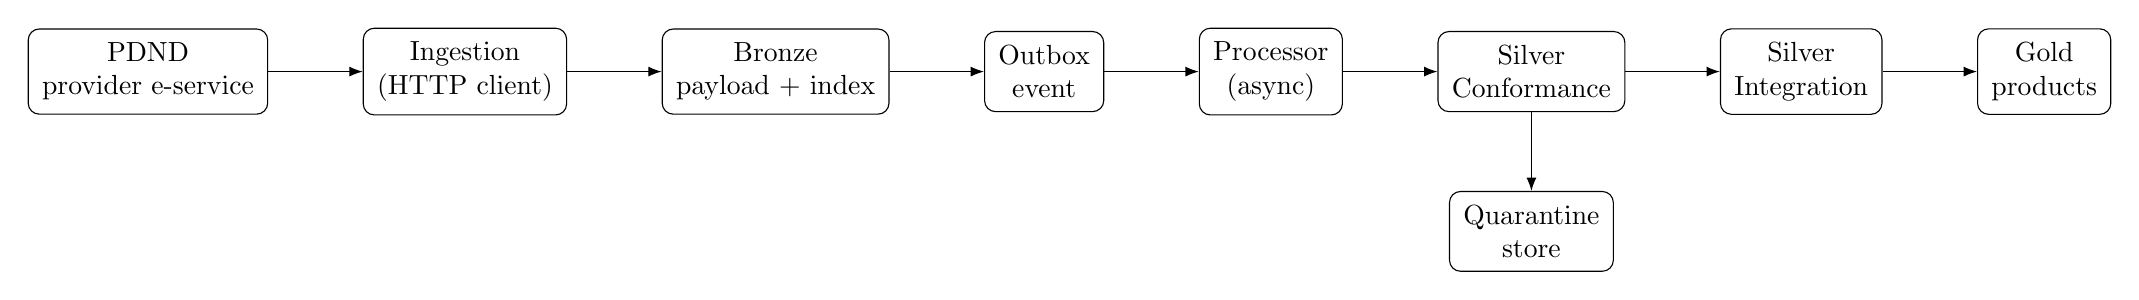
\begin{tikzpicture}[
  node distance=10mm and 12mm,
  box/.style={draw, rounded corners, inner sep=5pt, align=center},
  arr/.style={-Latex, line width=0.4pt}
]
\node[box] (pdnd) {PDND\\provider e-service};
\node[box, right=of pdnd] (ing) {Ingestion\\(HTTP client)};
\node[box, right=of ing] (bronze) {Bronze\\payload + index};
\node[box, right=of bronze] (outbox) {Outbox\\event};
\node[box, right=of outbox] (worker) {Processor\\(async)};
\node[box, right=of worker] (silverc) {Silver\\Conformance};
\node[box, below=of silverc] (quar) {Quarantine\\store};
\node[box, right=of silverc] (silverg) {Silver\\Integration};
\node[box, right=of silverg] (gold) {Gold\\products};

\draw[arr] (pdnd) -- (ing);
\draw[arr] (ing) -- (bronze);
\draw[arr] (bronze) -- (outbox);
\draw[arr] (outbox) -- (worker);
\draw[arr] (worker) -- (silverc);
\draw[arr] (silverc) -- (silverg);
\draw[arr] (silverg) -- (gold);
\draw[arr] (silverc) -- (quar);
\end{tikzpicture}
\end{adjustbox}
\caption{Consumer-side pipeline: Bronze evidence, outbox-triggered processing, Silver conformance and integration, and Gold publication.}
\label{fig:dotnet-dataflow}
\end{figure}

\subsection{Ingestion boundary: Bronze and outbox}
\textbf{Objective.} Persist each PDND response as immutable evidence and trigger downstream processing reliably.

\textbf{Guarantees.}
\begin{itemize}
  \item Evidence is stored before any processing side effects.
  \item Processing can be retried without losing the event that starts the pipeline.
  \item The same exchange can be replayed deterministically for audit or reprocessing.
\end{itemize}

Listings~\ref{lst:outbox-primitives}--\ref{lst:ingestion-service} show a minimal separation between payload storage (bytes) and an index row (metadata + pointer), plus an outbox message emitted in the same unit-of-work.

\begin{lstlisting}[style=csharp,caption={Outbox primitives and an explicit unit-of-work boundary.},label={lst:outbox-primitives}]
public sealed record OutboxMessage(
    string MessageId,
    string Type,
    DateTimeOffset OccurredAtUtc,
    string PayloadJson
);

public interface IOutbox
{
    ValueTask EnqueueAsync(OutboxMessage message, CancellationToken ct);
}

public interface IUnitOfWork
{
    ValueTask ExecuteAsync(Func<CancellationToken, ValueTask> action, CancellationToken ct);
}
\end{lstlisting}

\begin{lstlisting}[style=csharp,caption={Ingestion: persist Bronze pointer and enqueue a processing event.},label={lst:ingestion-service}]
public sealed record BronzeStoredEvent(string BronzeId);

public sealed class PdndIngestionService
{
    private readonly IBronzePayloadStore _payloadStore;
    private readonly IBronzeIndexStore _indexStore;
    private readonly IOutbox _outbox;
    private readonly IUnitOfWork _uow;

    public PdndIngestionService(
        IBronzePayloadStore payloadStore,
        IBronzeIndexStore indexStore,
        IOutbox outbox,
        IUnitOfWork uow)
    {
        _payloadStore = payloadStore;
        _indexStore = indexStore;
        _outbox = outbox;
        _uow = uow;
    }

    public async ValueTask<string> IngestAsync(
        PdndExchangeMetadata meta,
        byte[] payloadBytes,
        byte[] payloadHashSha256,
        CancellationToken ct)
    {
        var bronzeId = Guid.NewGuid().ToString("N");

        await _uow.ExecuteAsync(async uowCt =>
        {
            var payloadRef = await _payloadStore.PutAsync(payloadBytes, meta.ContentType, uowCt);

            var row = new BronzePointer(
                BronzeId: bronzeId,
                Meta: meta,
                PayloadRef: payloadRef,
                PayloadHashBase64: Convert.ToBase64String(payloadHashSha256)
            );

            await _indexStore.AppendAsync(row, uowCt);

            var evt = new BronzeStoredEvent(bronzeId);
            var msg = new OutboxMessage(
                MessageId: Guid.NewGuid().ToString("N"),
                Type: nameof(BronzeStoredEvent),
                OccurredAtUtc: DateTimeOffset.UtcNow,
                PayloadJson: System.Text.Json.JsonSerializer.Serialize(evt)
            );

            await _outbox.EnqueueAsync(msg, uowCt);
        }, ct);

        return bronzeId;
    }
}
\end{lstlisting}

\subsection{Idempotency: safe retries by design}
\textbf{Objective.} Make retries a normal operating mode and prevent duplicate side effects.

\textbf{Guarantees.}
\begin{itemize}
  \item Reprocessing the same exchange does not create inconsistent Silver/Gold states.
  \item The idempotency scope is explicit (per Bronze exchange, per integration window, etc.).
\end{itemize}

\begin{lstlisting}[style=csharp,caption={Idempotency keys: stable and source-aware.}]
public interface IIdempotencyStore
{
    ValueTask<bool> TryBeginAsync(string key, DateTimeOffset nowUtc, CancellationToken ct);
    ValueTask CompleteAsync(string key, DateTimeOffset nowUtc, CancellationToken ct);
}

public static class IdempotencyKeys
{
    public static string Conformance(string bronzeId, SourceIdentity source)
        => $"conformance:{source.Organization}:{source.EServiceId}:{source.ContractVersion}:{bronzeId}";

    public static string Integration(string entityKey, DateOnly day)
        => $"integration:{entityKey}:{day:yyyyMMdd}";
}
\end{lstlisting}

\subsection{Integration orchestrator: from conformed to integrated}
\textbf{Objective.} Treat integrated state as a computed artifact derived from conformed records and deterministic policies.

\textbf{Guarantees.}
\begin{itemize}
  \item Entity resolution decisions are explicit (including ``unresolved'').
  \item Survivorship is applied consistently and produces traceable provenance.
  \item Integration is idempotent within a defined time window.
\end{itemize}

\begin{lstlisting}[style=csharp,caption={Integration orchestrator: resolution, survivorship, persistence.}]
public interface IConformedStore
{
    IAsyncEnumerable<ConformedRecord> GetByEntityKeyAsync(string entityKey, CancellationToken ct);
}

public interface IIntegratedStore
{
    ValueTask UpsertAsync(IntegratedEntity entity, CancellationToken ct);
}

public sealed class IntegrationOrchestrator
{
    private readonly IEntityResolver _resolver;
    private readonly ISurvivorshipPolicy _survivorship;
    private readonly IConformedStore _conformed;
    private readonly IIntegratedStore _integrated;
    private readonly IIdempotencyStore _idempotency;

    public IntegrationOrchestrator(
        IEntityResolver resolver,
        ISurvivorshipPolicy survivorship,
        IConformedStore conformed,
        IIntegratedStore integrated,
        IIdempotencyStore idempotency)
    {
        _resolver = resolver;
        _survivorship = survivorship;
        _conformed = conformed;
        _integrated = integrated;
        _idempotency = idempotency;
    }

    public async ValueTask IntegrateAsync(ConformedRecord incoming, CancellationToken ct)
    {
        var now = DateTimeOffset.UtcNow;

        var decision = _resolver.ResolveEntityKey(incoming);
        if (decision.Confidence == MatchConfidence.Unresolved)
            return;

        var idKey = IdempotencyKeys.Integration(
            decision.EntityKey,
            DateOnly.FromDateTime(now.UtcDateTime));

        if (!await _idempotency.TryBeginAsync(idKey, now, ct))
            return;

        // Merge candidates deterministically and avoid duplicates (e.g., if the incoming record
        // is already present in the conformed store due to prior steps or retries).
        var byBronzeId = new Dictionary<string, ConformedRecord>(StringComparer.Ordinal);
        await foreach (var c in _conformed.GetByEntityKeyAsync(decision.EntityKey, ct))
            byBronzeId[c.BronzeId] = c;

        byBronzeId[incoming.BronzeId] = incoming;
        var candidates = byBronzeId.Values.ToList();

        var merged = _survivorship.Merge(decision.EntityKey, candidates, now);
        await _integrated.UpsertAsync(merged, ct);

        await _idempotency.CompleteAsync(idKey, now, ct);
    }
}
\end{lstlisting}

\section{Conclusion}
PDND is a strong enabler for interoperability, but interoperability becomes operational value only when exchanged information is trustworthy over time and usable across contexts.
In cross-administration scenarios, that value depends on the ability to integrate multiple sources with internal data while preserving lineage, handling conflicts consistently, and supporting controlled evolution.

A consumer-side Medallion lifecycle makes these requirements concrete: retain evidence, stabilize meaning, reconcile sources through explicit policies, and publish reusable products with stable contracts \cite{databricks_medallion_docs}.
Data quality becomes an engineering discipline grounded in consumer needs and explicit semantics \cite{wang_strong_1996,wand_wang_1996}.
Semantic interoperability strengthens reuse by making meaning explicit through semantic profiles and controlled vocabularies \cite{isa2_core_vocabularies,eu_vocabularies_controlled}.
Finally, record linkage foundations reinforce that entity resolution is a decision process with explicit trade-offs, not an incidental join \cite{fellegi_sunter_1969}.

\vspace{0.15cm}
\noindent\textbf{Source reference:} \cite{delre_medallion_pdnd_2026}

\printbibliography

\section*{Artifact availability}
The LaTeX sources, build instructions, and versioned releases for this paper are maintained at:
\url{https://github.com/engineering87/medallion-pdnd-paper}.

For reproducibility, each release is tagged in the repository and archived on Zenodo.
The recommended citation will reference the corresponding Git tag (e.g., \texttt{vX.Y.Z}) and the Zenodo DOI once available.
Build steps are provided in the header of the main \LaTeX{} source file and can be executed using \texttt{pdflatex} + \texttt{biber}.

\end{document}
